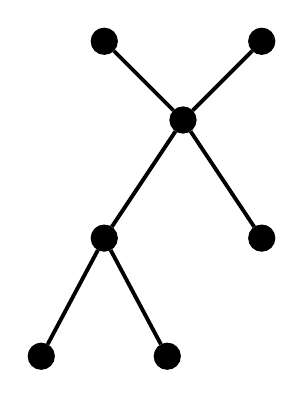
\begin{tikzpicture}

% NODES %%%%%%%%%%%%%%%%%%%%%%%%%%%%%%%%%%%%%%%%%%%%%%%%%%%%%%%%%%%%%%%%%%

\node[draw, circle, minimum height=0.2cm, minimum width=0.2cm, fill=black] (P0a) at (2,5) {};
\node[draw, circle, minimum height=0.2cm, minimum width=0.2cm, fill=black] (P0b) at (4,5) {};
\node[draw, circle, minimum height=0.2cm, minimum width=0.2cm, fill=black] (P1) at (3,4) {};
\node[draw, circle, minimum height=0.2cm, minimum width=0.2cm, fill=black] (P2) at (2,2.5) {};
\node[draw, circle, minimum height=0.2cm, minimum width=0.2cm, fill=black] (P3) at (4,2.5) {};
\node[draw, circle, minimum height=0.2cm, minimum width=0.2cm, fill=black] (P4) at (1.2,1) {};
\node[draw, circle, minimum height=0.2cm, minimum width=0.2cm, fill=black] (P5) at (2.8,1) {};


% LINKS %%%%%%%%%%%%%%%%%%%%%%%%%%%%%%%%%%%%%%%%%%%%%%%%%%%%%%%%%%%%%%%%%%

\draw[line width = 1.4pt] (P0a) -- (P1);
\draw[line width = 1.4pt] (P0b) -- (P1);
\draw[line width = 1.4pt] (P1) -- (P2);
\draw[line width = 1.4pt] (P1) -- (P3);
\draw[line width = 1.4pt] (P2) -- (P4);
\draw[line width = 1.4pt] (P2) -- (P5);

\end{tikzpicture}
